%% PCSJ(画像符号化シンポジウム) / IMPS(映像メディア情報シンポジウム) 用テンプレート
%% このテンプレートは「日本語向け」です.
%% 英語で論文を記述する場合は manuscript-english.tex を使用してください.
%
\documentclass[a4paper,10pt,dvipdfmx,twocolumn]{jsarticle}
% \documentclass[a4paper,10pt,dvipdfmx,twocolumn]{jarticle}

\usepackage{pcsjimps-j}
\usepackage[japanese]{ikelab-pcsjimps}

%!TEX encoding = UTF-8 Unicode
%
% 卒論 / 修論用 プリアンブル
%

%% フォント
\usepackage{lmodern}
\usepackage[scale=0.95]{tgheros}
\usepackage{textcomp}
\usepackage[scaled=0.85]{beramono}
\usepackage[T1]{fontenc}

%% パッケージ
\usepackage[cmex10]{amsmath}
\usepackage{amssymb,amsfonts,mathtools,bm}

\usepackage{graphicx,color}
\usepackage[table]{xcolor}

\usepackage[pdfborder={0 0 0}]{hyperref}
\usepackage{pxjahyper}

% caption のコロン「図4.4: キャプション」を「図4.4 キャプション」に直す
\usepackage[labelsep=quad,compatibility=false]{caption}
\usepackage[belowskip=1.2em]{subcaption}

\usepackage{cite,url,array,makecell}
\usepackage{algorithm,algorithmic}

% 数学コマンドの補完
\DeclareMathOperator*{\sinc}{sinc}
\DeclareMathOperator*{\prox}{prox}
\DeclareMathOperator*{\argmin}{argmin}
\DeclareMathOperator*{\argmax}{argmax}

% 参考文献表示スタイルを変更
\bibliographystyle{sieicej}

% 赤色を少し暗くする
\definecolor{red}{rgb}{0.75,0,0}

\makeatletter
   % アルゴリズム図キャプションの表記を「Algorithm」→「アルゴリズム」に
   \renewcommand{\ALG@name}{アルゴリズム}
\makeatother

% 修正箇所に色付けするコマンド
%
% ・ コマンド版
%   \fixed{修正箇所}
%
% ・ 環境版
%   \begin{fixedregion}
%      修正箇所
%   \end{fixedregion}
\newcommand{\fixed}[1]{#1} 
\newenvironment{fixedregion}{\ignorespaces}{\ignorespacesafterend}
% 下の 2 行をコメントアウトすることで色付けを無効化します
\renewcommand{\fixed}[1]{\textcolor{red}{#1}}
\renewenvironment{fixedregion}{\protect\leavevmode\color{red}\ignorespaces}{\ignorespacesafterend}

% 強調
\newcommand{\strong}[1]{\textcolor{red}{\textbf{#1}}}



%% 日本語タイトル
\jtitle{画像符号化シンポジウム・映像メディア処理\\シンポジウム講演予稿の書き方}

%% 英語タイトル
\etitle{How to Prepare a Camera-Ready Paper for Picture Coding Symposium of Japan and Image Media Processing Symposium}

%% 著者
\author{
   %% \JEAuthor{日本語名}{英語名}{この著者を表示するのに必要な幅}
   \JEAuthor{藤沢 貴典 $^\dag$}{Takanori Fujisawa$^\dag$}{.3\hsize}
   \JEAuthor{池原 雅章$^\dag$}{Masaaki Ikehara$^\dag$}{.3\hsize}
   %% 2つ目以降の所属がある場合
   % \JEAuthor{和文著者3$^\ddag$}{Author 3$^\ddag$}{.\hsize}
}

%% 所属
\affiliate{
   %% \JEAffiliation{日本語所属}{英語所属}{この所属を表示するのに必要な幅}
   \JEAffiliation{$^\dag$ 慶應義塾大学理工学部電子工学科}{$^\dag$ EEE Dept., Keio University}{.9\hsize}
   %% 2つ目以降の所属がある場合
   % \JEAffiliation{$^\ddag$和文所属2}{$^\ddag$English Affiliation 2}{.4\hsize}
}

%% 日本語概要
\begin{abstract}
  ここに日本語概要を300字程度で記述します.
%
本稿では非負値行列因子分解 (NMF) をベースにした楽曲の音高指定の手法を提案する.
NMF ベースの音高指定は短時間フーリエ変換によって得られた楽曲データの振幅スペクトログラムを,
その構成要素である楽器音の基底スペクトルおよび,その出現の線形結合の形に分解することで実現される.
この分離段階において,スペクトル方向には係数のスパース性が満たされ,
時間軸方向には滑らかに係数が出現しているのが望ましい.
著者は行列ノルム拘束を用いて,係数のスパース性と時間軸の連続性を同時に満足する手法を導入し,
それに基づく NMF 更新式を提案する.
この手法を用いたピアノ演奏データの音高推定を評価して,新しい NMF 手法が
入力スペクトル形状にロバストであり,またスペクトルの時間変化に強いことを示す.
\end{abstract}


\begin{document}

\pagestyle{empty}

\maketitle

\thispagestyle{empty}

%本文
\section{分量、原稿サイズ}

\begin{itemize}
\item 1件2ページ以内(図表を含む)
\item A4サイズ
\item 幅180mm
\item 高さ252mm
\item 段間の幅8mm程度(二段組の場合)
\end{itemize}
としてください。

\section{はじめに}
楽曲の音声信号は,楽器音,声,およびその他の信号の混ぜあわせとして表現される.
多声音高推定はこの音声信号を入力として,これら構成要素の基本周波数と,その時間変化を推定するものである.
この技術は楽曲の自動採譜やコード推定,特徴抽出といったアプリケーションへの応用が可能である.
従来の音高推定の手法としては correlogram を用いるもの \cite{pocsubimproved},
スペクトルピーククラスタリングを用いるもの\cite{pertusa2008},
サポートベクタマシンを用いるもの \cite{poliner2007} 等がある.

NMF (Non-negative Matrix Factorization : 非負値行列因子分解)はスペクトル分解の手法として
よく用いられているものの一つである.
これは音声信号のスペクトログラムを辞書行列と,その時間変化行列の積に分解する手法である.
NMF はその解が非負の値となるために,楽器ごとのパワースペクトルの加法性が近似的に成立する
音声信号処理との親和性が高い.また乗算更新則に基づく単純な計算で最適な解が得られる利点がある.

本稿では NMF をベースにした多声音高推定のアルゴリズムを提案する.
本手法は NMF によるスペクトル分離に対し実音楽に即した 2 つの特徴を組み込んでいる.
1 つ目は,出現するアクティベーションのピッチ方向のスパース性の確保であり,
もうひとつはアクティベーションの時間方向の連続性である.
両特徴を満たすために,本研究では行列ノルムを用いた結合スパース性拘束をアクティベーションに対して導入している.
この拘束条件の導入により,入力スペクトルが辞書行列中の基底に合わない部分での誤推定を減らす効果が期待される.
それに加え時間方向の連続性拘束は,入力スペクトル要素の時間的な変化に対して追従できる効果が期待される.

\subsection{NMF を用いた楽曲の音高推定}
50 $\sim$ 100 回の更新式適用によって得られたアクティベーション行列 $\bm{A}$ を元に
楽曲のピアノロール表現を作成する.
この際に,辞書 $\bm{S}$ の各インデックスが示す音高を推定する必要がある.
$\bm{S}$ の初期値に楽器音データベースから取得した基底スペクトルを用いた場合は,
該当する基底スペクトルの音高をそのまま用いることが出来る.

\subsubsection{スパース性と時間軸連続性拘束を付した NMF ベースの音高推定}

実音楽のデータに対し (\ref{eq:prev.updateA}) および (\ref{eq:prev.updateS}) 式の更新式で音高推定を行った場合,
アクティベーション行列 $\bm{A}$ において,実音楽の 2 つの特徴が無視される問題がある.
問題の 1 つめが,出現する基底インデックスのスパース性であり,
もう 1 つが,隣接するフレームのアクティベーション同士の連続性である.


\section{配置}


\begin{itemize}
\item 表題、著者名、勤務先は、本サンプルに従ってそれぞれ記入して下さい。
\item アブストラクト(和文の場合300字程度、英文の場合100語程度)をお入れ下さい。
\item 本文は一段または左右二段に書いても差し支えありません。
\item 用紙最終頁右下に、発表者連絡先をお入れ下さい(本サン
      プルのマクロ\verb|\simplefootnotetext|を使われると便利です)。
\end{itemize}



\section{文字サイズ}
文字サイズは、本サンプルを目安にしてください。
\begin{description}
\item[表題] 16ポイント (\verb|\LARGE|)
\item[和文著者名] 14ポイント(\verb|\Large|)
\item[英文著者名] 12ポイント(\verb|\large|)
\item[所属および本文] 10ポイント(\verb|\normalsize|)
\end{description}
程度です。

\section{図表}

\begin{table}[tb]
   \caption{符号化器の設定}
   \label{tab:settings}
   \centering
   \begin{tabular}{c||c|c}\hline
設定ア & aa & aaa\\\hline
設定イ & bb & bbb\\\hline
設定ウ & cc & ccc\\\hline
   \end{tabular}
\end{table}

\begin{figure}[tb]
   \centering
   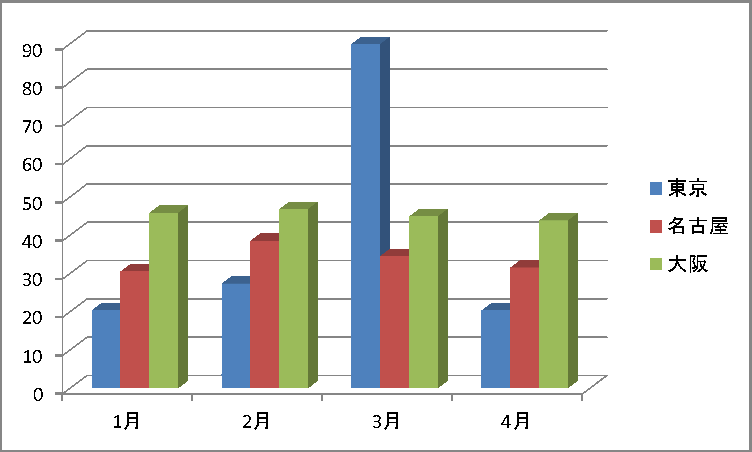
\includegraphics[width=.9\hsize]{figure/sample-j.pdf}\\
   \caption{符号化実験結果}
   \label{fig:results}
\end{figure}

予稿集は白黒・網がけ印刷になります。見にくくならないよう、作成の際には
ご注意ください。

図表の出力位置を指定するオプションは、[h]は使わず[t]、[b]などを指定して
ページの天か地に置くことを基本にします。

図表内は英文でも和文でも結構です。
参照は図\ref{fig:results}、表\ref{tab:settings}のようにしてください。

\bibliography{cites.bib}

\simplefootnotetext{
慶應義塾大学 電子工学科 池原研究室\\
〒{}223--8522 神奈川県横浜市港北区日吉4--5--33
Kohoku-ku, Yokohama, Kanagawa, 223--8522, Japan\\
E-mail: \url{ikehara@tkhm.elec.keio.ac.jp}}

\end{document}
